% Options for packages loaded elsewhere
\PassOptionsToPackage{unicode}{hyperref}
\PassOptionsToPackage{hyphens}{url}
%
\documentclass[
]{article}
\usepackage{lmodern}
\usepackage{amssymb,amsmath}
\usepackage{ifxetex,ifluatex}
\ifnum 0\ifxetex 1\fi\ifluatex 1\fi=0 % if pdftex
  \usepackage[T1]{fontenc}
  \usepackage[utf8]{inputenc}
  \usepackage{textcomp} % provide euro and other symbols
\else % if luatex or xetex
  \usepackage{unicode-math}
  \defaultfontfeatures{Scale=MatchLowercase}
  \defaultfontfeatures[\rmfamily]{Ligatures=TeX,Scale=1}
\fi
% Use upquote if available, for straight quotes in verbatim environments
\IfFileExists{upquote.sty}{\usepackage{upquote}}{}
\IfFileExists{microtype.sty}{% use microtype if available
  \usepackage[]{microtype}
  \UseMicrotypeSet[protrusion]{basicmath} % disable protrusion for tt fonts
}{}
\makeatletter
\@ifundefined{KOMAClassName}{% if non-KOMA class
  \IfFileExists{parskip.sty}{%
    \usepackage{parskip}
  }{% else
    \setlength{\parindent}{0pt}
    \setlength{\parskip}{6pt plus 2pt minus 1pt}}
}{% if KOMA class
  \KOMAoptions{parskip=half}}
\makeatother
\usepackage{xcolor}
\IfFileExists{xurl.sty}{\usepackage{xurl}}{} % add URL line breaks if available
\IfFileExists{bookmark.sty}{\usepackage{bookmark}}{\usepackage{hyperref}}
\hypersetup{
  pdftitle={Causal inquiries about a single unit},
  hidelinks,
  pdfcreator={LaTeX via pandoc}}
\urlstyle{same} % disable monospaced font for URLs
\usepackage[margin=1in]{geometry}
\usepackage{color}
\usepackage{fancyvrb}
\newcommand{\VerbBar}{|}
\newcommand{\VERB}{\Verb[commandchars=\\\{\}]}
\DefineVerbatimEnvironment{Highlighting}{Verbatim}{commandchars=\\\{\}}
% Add ',fontsize=\small' for more characters per line
\usepackage{framed}
\definecolor{shadecolor}{RGB}{248,248,248}
\newenvironment{Shaded}{\begin{snugshade}}{\end{snugshade}}
\newcommand{\AlertTok}[1]{\textcolor[rgb]{0.94,0.16,0.16}{#1}}
\newcommand{\AnnotationTok}[1]{\textcolor[rgb]{0.56,0.35,0.01}{\textbf{\textit{#1}}}}
\newcommand{\AttributeTok}[1]{\textcolor[rgb]{0.77,0.63,0.00}{#1}}
\newcommand{\BaseNTok}[1]{\textcolor[rgb]{0.00,0.00,0.81}{#1}}
\newcommand{\BuiltInTok}[1]{#1}
\newcommand{\CharTok}[1]{\textcolor[rgb]{0.31,0.60,0.02}{#1}}
\newcommand{\CommentTok}[1]{\textcolor[rgb]{0.56,0.35,0.01}{\textit{#1}}}
\newcommand{\CommentVarTok}[1]{\textcolor[rgb]{0.56,0.35,0.01}{\textbf{\textit{#1}}}}
\newcommand{\ConstantTok}[1]{\textcolor[rgb]{0.00,0.00,0.00}{#1}}
\newcommand{\ControlFlowTok}[1]{\textcolor[rgb]{0.13,0.29,0.53}{\textbf{#1}}}
\newcommand{\DataTypeTok}[1]{\textcolor[rgb]{0.13,0.29,0.53}{#1}}
\newcommand{\DecValTok}[1]{\textcolor[rgb]{0.00,0.00,0.81}{#1}}
\newcommand{\DocumentationTok}[1]{\textcolor[rgb]{0.56,0.35,0.01}{\textbf{\textit{#1}}}}
\newcommand{\ErrorTok}[1]{\textcolor[rgb]{0.64,0.00,0.00}{\textbf{#1}}}
\newcommand{\ExtensionTok}[1]{#1}
\newcommand{\FloatTok}[1]{\textcolor[rgb]{0.00,0.00,0.81}{#1}}
\newcommand{\FunctionTok}[1]{\textcolor[rgb]{0.00,0.00,0.00}{#1}}
\newcommand{\ImportTok}[1]{#1}
\newcommand{\InformationTok}[1]{\textcolor[rgb]{0.56,0.35,0.01}{\textbf{\textit{#1}}}}
\newcommand{\KeywordTok}[1]{\textcolor[rgb]{0.13,0.29,0.53}{\textbf{#1}}}
\newcommand{\NormalTok}[1]{#1}
\newcommand{\OperatorTok}[1]{\textcolor[rgb]{0.81,0.36,0.00}{\textbf{#1}}}
\newcommand{\OtherTok}[1]{\textcolor[rgb]{0.56,0.35,0.01}{#1}}
\newcommand{\PreprocessorTok}[1]{\textcolor[rgb]{0.56,0.35,0.01}{\textit{#1}}}
\newcommand{\RegionMarkerTok}[1]{#1}
\newcommand{\SpecialCharTok}[1]{\textcolor[rgb]{0.00,0.00,0.00}{#1}}
\newcommand{\SpecialStringTok}[1]{\textcolor[rgb]{0.31,0.60,0.02}{#1}}
\newcommand{\StringTok}[1]{\textcolor[rgb]{0.31,0.60,0.02}{#1}}
\newcommand{\VariableTok}[1]{\textcolor[rgb]{0.00,0.00,0.00}{#1}}
\newcommand{\VerbatimStringTok}[1]{\textcolor[rgb]{0.31,0.60,0.02}{#1}}
\newcommand{\WarningTok}[1]{\textcolor[rgb]{0.56,0.35,0.01}{\textbf{\textit{#1}}}}
\usepackage{graphicx,grffile}
\makeatletter
\def\maxwidth{\ifdim\Gin@nat@width>\linewidth\linewidth\else\Gin@nat@width\fi}
\def\maxheight{\ifdim\Gin@nat@height>\textheight\textheight\else\Gin@nat@height\fi}
\makeatother
% Scale images if necessary, so that they will not overflow the page
% margins by default, and it is still possible to overwrite the defaults
% using explicit options in \includegraphics[width, height, ...]{}
\setkeys{Gin}{width=\maxwidth,height=\maxheight,keepaspectratio}
% Set default figure placement to htbp
\makeatletter
\def\fps@figure{htbp}
\makeatother
\setlength{\emergencystretch}{3em} % prevent overfull lines
\providecommand{\tightlist}{%
  \setlength{\itemsep}{0pt}\setlength{\parskip}{0pt}}
\setcounter{secnumdepth}{-\maxdimen} % remove section numbering
\usepackage{booktabs}
\usepackage{longtable}
\usepackage{array}
\usepackage{multirow}
\usepackage{wrapfig}
\usepackage{float}
\usepackage{colortbl}
\usepackage{pdflscape}
\usepackage{tabu}
\usepackage{threeparttable}
\usepackage{threeparttablex}
\usepackage[normalem]{ulem}
\usepackage{makecell}
\usepackage{xcolor}

\title{Causal inquiries about a single unit}
\author{}
\date{\vspace{-2.5em}}

\begin{document}
\maketitle

\hypertarget{causal-inquiries-about-a-single-unit}{%
\subsection{Causal inquiries about a single
unit}\label{causal-inquiries-about-a-single-unit}}

We sometimes start a causal investigation wanting to know the causal
effect for a single unit. For example, for a unit that experienced an
event or process, we want to know the causal effect of that event. To do
so, we need to know what would have happened if the event did not
happen, the \emph{counter}factual outcome as opposed to the factual
outcome that actually occurred. Due to the fundamental problem of causal
inference, we cannot \emph{observe} what would have happened if that
counterfactual case had happened. We have to guess---or infer---what
would have happened. Social scientists have developed a large array of
tools for guessing missing counterfactual outcomes --- what would have
happened in the counterfactual case, if the event had not
happened.\footnote{We are also interested in the opposite case
  sometimes: we have a unit that did not experience an event, and we
  want to know the causal effect of \emph{not} having it. In this case,
  we need to guess what would have happened if the event did happen. The
  same tools apply in reverse.}

A common estimand in this setting is whether an outcome was \emph{due}
to a cause. This ``attribution'' estimand or ``Cause of Effect''
estimand can be written \(CoE:=1-Y(0)| X=1 \text{ \& } Y=1\). For a unit
with \(X=1\) and \(Y=1\), \(CoE=1\) if \(Y(0)=0\). One might also be
interested in the treatment effect of the treated case (TET). The TET is
the difference between the treated potential outcome and the control
potential outcome in the posttreatment period for the treated unit of
interest---but not conditioning on knowledge of the outcome.

\hypertarget{process-tracing}{%
\subsubsection{Process tracing}\label{process-tracing}}

``Process tracing'' is a prominent strategy for assessing causes of
effects (Bennett and Checkel 2015; Fairfield and Charman 2017). Here,
following for example Humphreys and Jacobs (2017), we think of process
tracing as a procedure in which researchers provide a theory, in the
form of a causal model, that is rich enough to characterize the
probability of observing ancillary data (``Causal process observations''
(Brady 2004)) given underlying causal relations. If equipped with
priors, such a model in turn lets one use Bayes' rule to form posteriors
over causal relations when these observations are observed.

For intuition, say we are interested in whether a policy caused a change
in economic outcomes. We expect that for the policy to matter it at
least had to be implemented and so if we find out that it was not
implemented we infer that it did not matter. Thus we make theory
dependent inferences that are reasonable \emph{insofar as} the theory is
reasonable. In this example, if there are plausible channels through
which a policy might have mattered even if not implmenented, then our
conclusion would not be warranted.

To illustrate design choices for a process tracing study we consider a
setting in which we have observed \(X=1\) and \(Y=1\) and we are
interested in figuring out whether \(Y=1\) \emph{because} \(X=1\). More
specifically we imagine a model with two ancillary variables, \(M\) and
\(W\). We posit that \(X\) causes \(Y\) via \(M\)---with negative
effects of \(X\) on \(M\) and of \(M\) and \(Y\) ruled out. And we posit
that \(W\) is a cause of both \(M\) and \(Y\), specifically we posit
that if \(W=1\) then \(X\) causes \(M\) and \(M\) causes \(Y\) for sure.
Under this model \(M\) and \(W\) each serve as ``clues'' for the causal
effect of \(X\) on \(Y\). Using the language popularized by Van Evera
(1997), \(M\) provides a ``hoop'' test---if you look for data on \(M\)
and find that \(M=0\) then you infer that \(X\) did not cause \(Y\); if
on the other hand you examine \(W\) and find that \(W=1\) then you have
a ``smoking gun'' test and you infer that \(X\) did indeed cause \(Y\).
If you find both \(M=0\) and \(W=1\) then you know your model is wrong.

The model can be described using the \texttt{CausalQueries} package
thus:

\begin{Shaded}
\begin{Highlighting}[]
\NormalTok{model <-}\StringTok{ }\KeywordTok{make_model}\NormalTok{(}\StringTok{"X -> M -> Y <- W -> M"}\NormalTok{) }\OperatorTok
\StringTok{  }\KeywordTok{set_restrictions}\NormalTok{(}\StringTok{"(M[X=1] < M[X=0]) | (M[X=1, W=1] == M[X=0, W=1])"}\NormalTok{) }\OperatorTok
\StringTok{  }\KeywordTok{set_restrictions}\NormalTok{(}\StringTok{"(Y[M=1] < Y[M=0]) | (Y[M=1, W=1] == Y[M=0, W=1])"}\NormalTok{)}

\KeywordTok{plot}\NormalTok{(model)}
\end{Highlighting}
\end{Shaded}

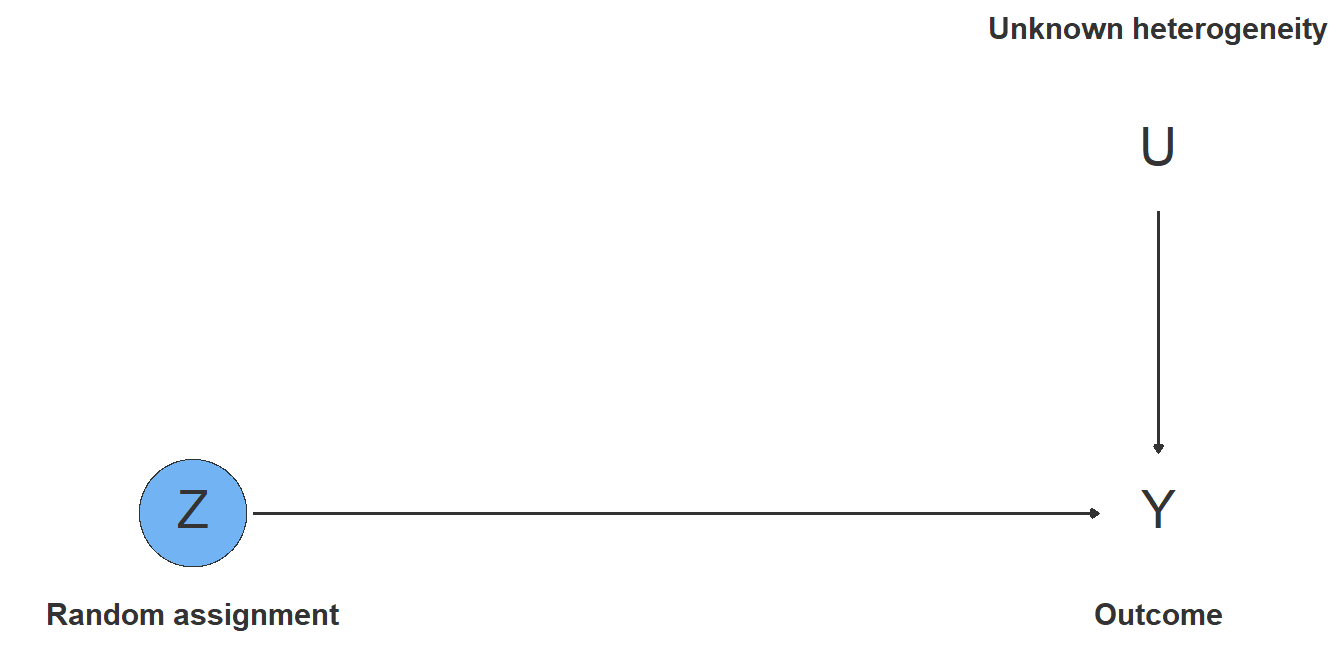
\includegraphics{02_Single_Case_Inquiries_files/figure-latex/unnamed-chunk-5-1.pdf}

This model definition describes the DAG but also specifies a set of
restrictions on causal relations. By default flat priors are then placed
over all other possible causal relations, though other prior beliefs
could also be specified.

We now have all we need to assess what inferences we might make given
different sorts of observations using
\texttt{CausalQueries::query\_model}. This function lets you ask any
causal question of of a model conditional on observed (or
counterfactual) conditions. We can use it to calculate beliefs, likely
data, and conditional inferences thus:

\begin{Shaded}
\begin{Highlighting}[]
\NormalTok{queries <-}\StringTok{ }
\StringTok{  }\NormalTok{CausalQueries}\OperatorTok{::}\KeywordTok{query_model}\NormalTok{(}
\NormalTok{    model,}
    \DataTypeTok{query =} \KeywordTok{list}\NormalTok{(}\StringTok{'Prob(CoE=1)'}\NormalTok{ =}\StringTok{ "Y[X=1] > Y[X=0]"}\NormalTok{,}
                 \StringTok{'Prob(M=1)'}\NormalTok{ =}\StringTok{ "M==1"}\NormalTok{,}
                 \StringTok{'Prob(CoE=1 | M=0)'}\NormalTok{ =}\StringTok{ "Y[X=1] > Y[X=0]"}\NormalTok{,}
                 \StringTok{'Prob(CoE=1 | M=1)'}\NormalTok{ =}\StringTok{ "Y[X=1] > Y[X=0]"}\NormalTok{),}
    \DataTypeTok{given =} \KeywordTok{list}\NormalTok{(}\StringTok{"Y==1 & X==1"}\NormalTok{,}
                 \StringTok{"Y==1 & X==1"}\NormalTok{,}
                 \StringTok{"Y==1 & X==1 & M==0"}\NormalTok{,}
                 \StringTok{"Y==1 & X==1 & M==1"}\NormalTok{),}
    \DataTypeTok{using =} \StringTok{"parameters"}\NormalTok{) }
\end{Highlighting}
\end{Shaded}

\begin{table}

\caption{\label{tab:ptprobative}Beliefs for a case with $X=1, Y=1$. The first row gives the prior belief that $X=1$ caused $Y=1$.  The second row gives the expecation that M=1. The last rows gives posterior beliefs that X=1 caused Y=1 after M is observed, depending on what is found.}
\centering
\begin{tabular}[t]{l|l|r}
\hline
Query & Given & mean\\
\hline
Prob(CoE=1) & Y==1 \& X==1 & 0.71\\
\hline
Prob(M=1) & Y==1 \& X==1 & 0.93\\
\hline
Prob(CoE=1 | M=0) & Y==1 \& X==1 \& M==0 & 0.00\\
\hline
Prob(CoE=1 | M=1) & Y==1 \& X==1 \& M==1 & 0.77\\
\hline
\end{tabular}
\end{table}

From the model specification, we can calculate directly the probability
of observing \(M=0\) or \(M=1\) (or \(W=0\) or \(W=1\)) and what we
would infer in each case. Table @ref(tab:ptprobative) shows an example
of these values. From a table like this we can calculate directly the
expected posterior variance associated with a process tracing data
strategy and a Bayesian answer strategy. For instance, here our prior on
CoE is 0.71 which implies a variance of 0.2. If we gather data on \(M\)
however our posterior variance will be either 0.18 (with probability
0.93) or 0.

Thus we see that we can already imagine how our a design in which we
seek data on \(M\) only will perform in expectation in terms of reducing
our uncertainty. No simulation is required. Even still, we think it
useful to fold these quantities into a design declaration so that users
can access the data strategies and answer strategies in the same way as
they would for any other problem.

The design declaration below uses a custom data function that draws a
value of the estimand (EoC) using the prior in the first row of Table
@ref(tab:ptprobative) and then draws values of \(M\), using values from
the second row of Table @ref(tab:ptprobative) (and similarly for \(W\)).
The estimation step also uses a custom function, which simply returns
the posterior estimates---like those in the last rows of Table
@ref(tab:ptprobative), but for both \(M\) and \(W\). No data strategy is
provided because we imagine estimation given all possible data
strategies (observation of \(M\), of \(W\), and of both).

\begin{Shaded}
\begin{Highlighting}[]
\NormalTok{design <-}\StringTok{ }
\StringTok{  }\KeywordTok{declare_population}\NormalTok{(}\DataTypeTok{data =} \KeywordTok{data_function}\NormalTok{()) }\OperatorTok{+}\StringTok{ }
\StringTok{  }\KeywordTok{declare_inquiry}\NormalTok{(}\DataTypeTok{CoE =}\NormalTok{ CoE) }\OperatorTok{+}
\StringTok{  }\KeywordTok{declare_estimator}\NormalTok{(}\DataTypeTok{handler =}\NormalTok{ my_estimator_function)}
\end{Highlighting}
\end{Shaded}

Given such a model, a case in which \(X=Y=1\), and limited resources, we
now want to know whether we would be better gathering data on \(M\) or
on \(W\) or both? The answers are given in Table @ref(tab:ptdiagnosis).
We see only modest declines in expected posterior variance from
observation of the mediator \(M\), consistent with the manual
calculation above; but large declines from observing \(W\).

Note here that model used for \(M\) and \(M\) is the same model used for
\(A\). This does not \emph{have} to be the case however. If instead we
used different models in these two parts we could assess how well or
poorly our strategy performs when our model is wrong. In this case, and
unlike the results in table @ref(tab:ptdiagnosis) we woudl find that hte
expected posterior variance (where the expectation is taken with respect
to the model in \(M\) but posterior taken with respect to the model in
\(A\)) will not be the same as the expected mean squared error. Can you
see why not?

\begin{table}

\caption{\label{tab:ptdiagnosis}Inference upon observation of $M$ or $W$ for cases in which $X = 1$ and $Y = 1$. We see that expected posterior variance (equivalently, expected mean squared error) falls modestly when $M$ is observed but substantially when $W$ is observed. The gains from observing $W$ are modest if $M$ is already observed.}
\centering
\begin{tabular}[t]{l|l|l|l|l|l|l|l}
\hline
Estimand Label & Estimator Label & N Sims & Bias & Mse & Mean Posterior Var & Mean Estimate & Mean Estimand\\
\hline
CoE & Prior & 1000 & 0.01 & 0.21 & 0.20 & 0.71 & 0.70\\
\hline
 &  &  & (0.01) & (0.01) & (0.00) & (0.00) & (0.01)\\
\hline
CoE & M only & 1000 & 0.01 & 0.17 & 0.16 & 0.71 & 0.70\\
\hline
 &  &  & (0.01) & (0.01) & (0.00) & (0.01) & (0.01)\\
\hline
CoE & W only & 1000 & 0.00 & 0.06 & 0.06 & 0.71 & 0.70\\
\hline
 &  &  & (0.01) & (0.01) & (0.00) & (0.01) & (0.01)\\
\hline
CoE & Both & 1000 & 0.00 & 0.05 & 0.06 & 0.71 & 0.70\\
\hline
 &  &  & (0.01) & (0.00) & (0.00) & (0.01) & (0.01)\\
\hline
\end{tabular}
\end{table}

\hypertarget{before-after-comparison}{%
\subsubsection{Before-after comparison}\label{before-after-comparison}}

A natural idea for guessing what would have happened if an event did not
occur for a single unit is to look within that unit at what happened
\emph{before} the event did occur. Within-unit over-time comparisons use
outcomes in pretreatment periods to impute the posttreatment
counterfactual outcome.

In order for the pretreatment outcome to be a good stand-in for the
posttreatment control potential outcome, we must invoke two assumptions:
excludability of time; and no interference between time periods. The
excludability assumption says that the only change between pre and post
is the fact that the treatment is administered. This rules out time
trends and any other form of time-varying heterogeneity aside from the
treatment status. The second assumption is that the unit is assigned to
control in the pretreatment period cannot affect outcomes in the
posttreatment period, and the fact that the unit is treated in the
second period cannot affect outcomes in the first period. This is often
called a no carryover assumption, and most importantly in this case
rules out the possibility of effects of anticipating treatment in the
next period. If the unit expects to be treated in period 1, this may
affect the outcome in period 0 even though treatment has not yet been
administered. Often anticipation effects wash out treatment effects; it
is as if the treatment has already taken place.

To declare this design, we consider violations of the excludability
assumption. The inquiry is the TET, as in all designs in this section.
In the model, we consider two sources of heterogeneity in the outcome:
time trends (an effect of time) and time-varying heterogeneity (an
effect of \(U_{\rm time}\)). Potential outcomes are a function of these
two variables and the treatment variable. Our data strategy is to
measure \(Y\) in both periods, and this will reveal the control
potential outcome in the first period, before treatment, and the control
potential outcome in the second period, after treatment. Our answer
strategy is to take the difference in the outcome between the post- and
pretreatment periods.

\begin{Shaded}
\begin{Highlighting}[]
\NormalTok{design <-}\StringTok{ }
\StringTok{  }\KeywordTok{declare_population}\NormalTok{(}
    \DataTypeTok{N =} \DecValTok{2}\NormalTok{, }
    \DataTypeTok{time =} \DecValTok{0}\OperatorTok{:}\DecValTok{1}\NormalTok{,}
    \DataTypeTok{U_time =} \KeywordTok{rnorm}\NormalTok{(N),}
    \KeywordTok{potential_outcomes}\NormalTok{(}
\NormalTok{      Y }\OperatorTok{~}\StringTok{ }\NormalTok{time_trend }\OperatorTok{*}\StringTok{ }\NormalTok{time }\OperatorTok{+}\StringTok{ }\NormalTok{time_specific_effect }\OperatorTok{*}\StringTok{ }\NormalTok{U_time }\OperatorTok{+}\StringTok{ }\FloatTok{0.5} \OperatorTok{*}\StringTok{ }\NormalTok{Z}
\NormalTok{    ),}
    \DataTypeTok{Z =} \DecValTok{1}
\NormalTok{  ) }\OperatorTok{+}\StringTok{ }
\StringTok{  }\KeywordTok{declare_inquiry}\NormalTok{(}\DataTypeTok{TET =}\NormalTok{ Y_Z_}\DecValTok{1} \OperatorTok{-}\StringTok{ }\NormalTok{Y_Z_}\DecValTok{0}\NormalTok{, }\DataTypeTok{subset =}\NormalTok{ time }\OperatorTok{==}\StringTok{ }\DecValTok{1}\NormalTok{) }\OperatorTok{+}\StringTok{ }
\StringTok{  }\KeywordTok{declare_measurement}\NormalTok{(}\DataTypeTok{Y =} \KeywordTok{ifelse}\NormalTok{(time }\OperatorTok{==}\StringTok{ }\DecValTok{0}\NormalTok{, Y_Z_}\DecValTok{0}\NormalTok{, Y_Z_}\DecValTok{1}\NormalTok{)) }\OperatorTok{+}\StringTok{ }
\StringTok{  }\KeywordTok{declare_estimator}\NormalTok{(}
    \DataTypeTok{estimate =}\NormalTok{ Y[time }\OperatorTok{==}\StringTok{ }\DecValTok{1}\NormalTok{] }\OperatorTok{-}\StringTok{ }\NormalTok{Y[time }\OperatorTok{==}\StringTok{ }\DecValTok{0}\NormalTok{], }
    \DataTypeTok{estimand_label =} \StringTok{"TET"}\NormalTok{, }\DataTypeTok{handler =}\NormalTok{ summarize)}

\NormalTok{designs <-}\StringTok{ }\KeywordTok{redesign}\NormalTok{(}
\NormalTok{  design, }\DataTypeTok{time_trend =} \KeywordTok{c}\NormalTok{(}\DecValTok{0}\NormalTok{, }\FloatTok{0.5}\NormalTok{), }\DataTypeTok{time_specific_effect =} \KeywordTok{c}\NormalTok{(}\DecValTok{0}\NormalTok{, }\DecValTok{1}\NormalTok{))}
\end{Highlighting}
\end{Shaded}

\begin{Shaded}
\begin{Highlighting}[]
\NormalTok{diagnosis <-}\StringTok{ }\KeywordTok{diagnose_design}\NormalTok{(designs, }\DataTypeTok{sims =}\NormalTok{ sims, }\DataTypeTok{bootstrap_sims =}\NormalTok{ b_sims)}
\end{Highlighting}
\end{Shaded}

We diagnose the design in four settings, the two-by-two of: with and
without time trends, and with and without time-specific effects. We see
that the over-time within-unit design is only unbiased when there are
neither. If there are time trends, there is bias, due to a violation of
the excludability of time assumption. If there is time-varying
heterogeneity aside from the treatment, the excludability assumption is
also violated. There is no test for these two conditions that lead to
bias, and there is no diagnostic like the pretrends comparison for the
difference-in-difference design.

\begin{tabular}{rrrr}
\toprule
time\_trend & time\_specific\_effect & bias & se(bias)\\
\midrule
0.0 & 0 & 0.000 & 0.00\\
0.5 & 0 & 0.500 & 0.00\\
0.0 & 1 & -0.011 & 0.02\\
0.5 & 1 & 0.470 & 0.02\\
\bottomrule
\end{tabular}

\hypertarget{posttreatment-comparison-to-an-untreated-case}{%
\subsubsection{Posttreatment comparison to an untreated
case}\label{posttreatment-comparison-to-an-untreated-case}}

A second natural design is to compare the outcomes of the treated case
after to treatment to the outcomes in another unit in the same time
period that did not receive the treatment. Instead of filling in the
control potential outcome of the treated unit with its own outcome in
the pretreatment period, we fill it in with the outcomes of this second
``control'' unit.

We can invoke an exactly parallel set of assumptions to the over time
within unit design: excludability of the unit difference (rather than
time), i.e., the only difference between the two units is the treatment
status and not other unit-specific heterogeneity. This strong assumption
is often relaxed in favor of a ``selection-on-observables'' assumption
by accounting for observable differences between units and selecting a
comparison unit that is similar in all observable ways.

In declaring the design, we target the same TET inquiry, and swap our
model of over time heterogeneity with with between-unit heterogeneity
(\(U_{\rm unit}\)) (there is not a parallel of time trends). Our data
strategy is to measure Y for both the treated unit and the comparison
unit in the posttreatment time period; the treated unit reveals its
treated potential outcome, while the comparison unit reveals its control
potential outcome. The answer strategy is the posttreatment comparison
between the treated and control unit.

\begin{Shaded}
\begin{Highlighting}[]
\NormalTok{design <-}\StringTok{ }
\StringTok{  }\KeywordTok{declare_population}\NormalTok{(}
    \DataTypeTok{N =} \DecValTok{2}\NormalTok{, }
    \DataTypeTok{time =} \DecValTok{1}\NormalTok{,}
    \DataTypeTok{U_unit =} \KeywordTok{rnorm}\NormalTok{(N),}
    \KeywordTok{potential_outcomes}\NormalTok{(Y }\OperatorTok{~}\StringTok{ }\FloatTok{0.5} \OperatorTok{*}\StringTok{ }\NormalTok{Z }\OperatorTok{+}\StringTok{ }\NormalTok{unit_specific_effect }\OperatorTok{*}\StringTok{ }\NormalTok{U_unit),}
    \DataTypeTok{Z =} \KeywordTok{if_else}\NormalTok{(U_unit }\OperatorTok{==}\StringTok{ }\KeywordTok{max}\NormalTok{(U_unit), }\DecValTok{1}\NormalTok{, }\DecValTok{0}\NormalTok{)}
\NormalTok{  ) }\OperatorTok{+}\StringTok{ }
\StringTok{  }\KeywordTok{declare_inquiry}\NormalTok{(}\DataTypeTok{TET =}\NormalTok{ Y_Z_}\DecValTok{1} \OperatorTok{-}\StringTok{ }\NormalTok{Y_Z_}\DecValTok{0}\NormalTok{, }\DataTypeTok{subset =}\NormalTok{ time }\OperatorTok{==}\StringTok{ }\DecValTok{1}\NormalTok{) }\OperatorTok{+}\StringTok{ }
\StringTok{  }\KeywordTok{declare_measurement}\NormalTok{(}\DataTypeTok{Y =} \KeywordTok{ifelse}\NormalTok{(Z }\OperatorTok{==}\StringTok{ }\DecValTok{0}\NormalTok{, Y_Z_}\DecValTok{0}\NormalTok{, Y_Z_}\DecValTok{1}\NormalTok{)) }\OperatorTok{+}\StringTok{ }
\StringTok{  }\KeywordTok{declare_estimator}\NormalTok{(}
    \DataTypeTok{estimate =}\NormalTok{ Y[Z }\OperatorTok{==}\StringTok{ }\DecValTok{1}\NormalTok{] }\OperatorTok{-}\StringTok{ }\NormalTok{Y[Z }\OperatorTok{==}\StringTok{ }\DecValTok{0}\NormalTok{], }
    \DataTypeTok{estimand_label =} \StringTok{"TET"}\NormalTok{, }\DataTypeTok{handler =}\NormalTok{ summarize)}

\NormalTok{designs <-}\StringTok{ }\KeywordTok{redesign}\NormalTok{(design, }\DataTypeTok{unit_specific_effect =} \KeywordTok{c}\NormalTok{(}\DecValTok{0}\NormalTok{, }\DecValTok{1}\NormalTok{))}
\end{Highlighting}
\end{Shaded}

\begin{Shaded}
\begin{Highlighting}[]
\NormalTok{diagnosis <-}\StringTok{ }\KeywordTok{diagnose_design}\NormalTok{(designs, }\DataTypeTok{sims =}\NormalTok{ sims, }\DataTypeTok{bootstrap_sims =}\NormalTok{ b_sims)}
\end{Highlighting}
\end{Shaded}

We diagnose the two-unit posttreatment comparison design under two
settings: with and without unit-specific differences not accounted for
by observables, aside from the treatment. With these differences, the
excludability assumption is violated. We see that the design is only
unbiased for the TET if there are no such unit-specific differences
besides treatment.

\begin{tabular}{rrr}
\toprule
unit\_specific\_effect & bias & se(bias)\\
\midrule
0 & 0.000 & 0.000\\
1 & 1.154 & 0.012\\
\bottomrule
\end{tabular}

\hypertarget{difference-in-differences}{%
\subsubsection{Difference-in-differences}\label{difference-in-differences}}

When the over-time excludability of treatment and the
selection-on-observables assumptions are unreasonable, an alternative is
the difference-in-differences design. We difference out unit
characteristics, whether observable or not, that do not vary over time
by comparing the outcomes before and after treatment. What is left is
time trends and other unit-invariant time-varying factors, and we
difference these out by comparing the change over time in the treated
unit to the change over time in the comparison unit. Each difference
takes out one class of factors that would violate the excludability
assumptions of over-time within unit designs alone or posttreatment
comparison across-unit designs alone.

The difference-in-difference design does not rely on the assumptions the
earlier two designs do. But it adds a new assumption: the parallel
trends assumption. In order for the difference-in-difference design to
work, the change between before and after treatment in the control
potential outcomes must be equal (i.e., parallel). Because this
assumption depends on the change in values of the unrealized (and thus
unobservable) control potential outcome in the treated unit, it cannot
be tested. There is a widely-used diagnostic of the difference in
observed trends before treatment {[}\ldots{]}

Declaring this design combines the elements of the within-unit over time
and between-unit posttreatment designs. We have two units (the treated
unit and its comparison unit), and two time periods, before (0) and
after treatment (1). There is unit-specific, time invariant
heterogeneity (\(U_{\rm unit}\)), and unit-invariant over time
heterogeneity (\(U_{\rm time}\)). The potential outcomes are a function
of treatment, these heterogeneity variables, and time trends. We target
the same TET inquiry as the other designs. We measure the outcome in a
way that combines the two previous designs: the control potential
outcome is revealed in both periods for the comparison untreated unit
\emph{and} in the pretreatmetn period for the treated unit, and the
treated potential outocme is revealed in the posttreatment period of the
treated unit. The answer strategy is the difference-in-differences,
first differencing off within-unit changes from first to second period
then across-unit changes in the comparison unit.

\begin{Shaded}
\begin{Highlighting}[]
\NormalTok{design <-}\StringTok{ }
\StringTok{  }\KeywordTok{declare_population}\NormalTok{(}
    \DataTypeTok{unit =} \KeywordTok{add_level}\NormalTok{(}\DataTypeTok{N =} \DecValTok{2}\NormalTok{, }\DataTypeTok{U_unit =} \KeywordTok{rnorm}\NormalTok{(N, }\DataTypeTok{sd =} \FloatTok{0.5}\NormalTok{), }\DataTypeTok{Z =} \KeywordTok{if_else}\NormalTok{(U_unit }\OperatorTok{==}\StringTok{ }\KeywordTok{max}\NormalTok{(U_unit), }\DecValTok{1}\NormalTok{, }\DecValTok{0}\NormalTok{)),}
    \DataTypeTok{period =} \KeywordTok{add_level}\NormalTok{(}\DataTypeTok{N =} \DecValTok{2}\NormalTok{, }\DataTypeTok{time =} \DecValTok{0}\OperatorTok{:}\DecValTok{1}\NormalTok{, }\DataTypeTok{U_time =} \KeywordTok{rnorm}\NormalTok{(N), }\DataTypeTok{nest =} \OtherTok{FALSE}\NormalTok{),}
    \DataTypeTok{unit_period =} \KeywordTok{cross_levels}\NormalTok{(}
      \DataTypeTok{by =} \KeywordTok{join}\NormalTok{(unit, period), }
      \DataTypeTok{U =} \KeywordTok{rnorm}\NormalTok{(N, }\DataTypeTok{sd =} \FloatTok{0.01}\NormalTok{),}
      \KeywordTok{potential_outcomes}\NormalTok{(}
\NormalTok{        Y }\OperatorTok{~}\StringTok{ }\NormalTok{time_trend }\OperatorTok{*}\StringTok{ }\FloatTok{0.5} \OperatorTok{*}\StringTok{ }\NormalTok{time }\OperatorTok{+}\StringTok{ }
\StringTok{          }\NormalTok{time_specific_effect }\OperatorTok{*}\StringTok{ }\NormalTok{U_time }\OperatorTok{+}\StringTok{ }
\StringTok{          }\NormalTok{unit_specific_effect }\OperatorTok{*}\StringTok{ }\NormalTok{U_unit }\OperatorTok{+}\StringTok{ }
\StringTok{          }\FloatTok{1.25} \OperatorTok{*}\StringTok{ }\NormalTok{Z }\OperatorTok{+}\StringTok{ }\NormalTok{U)}
\NormalTok{    )}
\NormalTok{  ) }\OperatorTok{+}\StringTok{ }
\StringTok{  }\KeywordTok{declare_inquiry}\NormalTok{(}\DataTypeTok{TET =}\NormalTok{ Y_Z_}\DecValTok{1} \OperatorTok{-}\StringTok{ }\NormalTok{Y_Z_}\DecValTok{0}\NormalTok{, }\DataTypeTok{subset =}\NormalTok{ time }\OperatorTok{==}\StringTok{ }\DecValTok{1}\NormalTok{) }\OperatorTok{+}\StringTok{ }
\StringTok{  }\KeywordTok{declare_measurement}\NormalTok{(}\DataTypeTok{Y =} \KeywordTok{if_else}\NormalTok{(Z }\OperatorTok{==}\StringTok{ }\DecValTok{0} \OperatorTok{|}\StringTok{ }\NormalTok{period }\OperatorTok{==}\StringTok{ }\DecValTok{1}\NormalTok{, Y_Z_}\DecValTok{0}\NormalTok{, Y_Z_}\DecValTok{1}\NormalTok{)) }\OperatorTok{+}\StringTok{ }
\StringTok{  }\KeywordTok{declare_estimator}\NormalTok{(}
    \DataTypeTok{estimate =} 
\NormalTok{      (}\KeywordTok{mean}\NormalTok{(Y[Z }\OperatorTok{==}\StringTok{ }\DecValTok{1} \OperatorTok{&}\StringTok{ }\NormalTok{time }\OperatorTok{==}\StringTok{ }\DecValTok{2}\NormalTok{]) }\OperatorTok{-}\StringTok{ }\KeywordTok{mean}\NormalTok{(Y[Z }\OperatorTok{==}\StringTok{ }\DecValTok{1} \OperatorTok{&}\StringTok{ }\NormalTok{time }\OperatorTok{==}\StringTok{ }\DecValTok{1}\NormalTok{])) }\OperatorTok{-}\StringTok{ }
\StringTok{      }\NormalTok{(}\KeywordTok{mean}\NormalTok{(Y[Z }\OperatorTok{==}\StringTok{ }\DecValTok{0} \OperatorTok{&}\StringTok{ }\NormalTok{time }\OperatorTok{==}\StringTok{ }\DecValTok{2}\NormalTok{]) }\OperatorTok{-}\StringTok{ }\KeywordTok{mean}\NormalTok{(Y[Z }\OperatorTok{==}\StringTok{ }\DecValTok{0} \OperatorTok{&}\StringTok{ }\NormalTok{time }\OperatorTok{==}\StringTok{ }\DecValTok{1}\NormalTok{])), }
    \DataTypeTok{estimand_label =} \StringTok{"ATT"}\NormalTok{, }\DataTypeTok{handler =}\NormalTok{ summarize)}

\NormalTok{designs <-}\StringTok{ }\KeywordTok{redesign}\NormalTok{(design, }
                    \DataTypeTok{time_trend =} \KeywordTok{c}\NormalTok{(}\DecValTok{0}\NormalTok{, }\FloatTok{0.5}\NormalTok{), }
                    \DataTypeTok{time_specific_effect =} \KeywordTok{c}\NormalTok{(}\DecValTok{0}\NormalTok{, }\DecValTok{1}\NormalTok{), }
                    \DataTypeTok{unit_specific_effect =} \KeywordTok{c}\NormalTok{(}\DecValTok{0}\NormalTok{, }\DecValTok{1}\NormalTok{))}
\end{Highlighting}
\end{Shaded}

\begin{Shaded}
\begin{Highlighting}[]
\NormalTok{diagnosis <-}\StringTok{ }\KeywordTok{diagnose_design}\NormalTok{(designs, }\DataTypeTok{sims =}\NormalTok{ sims, }\DataTypeTok{bootstrap_sims =}\NormalTok{ b_sims)}
\end{Highlighting}
\end{Shaded}

We diagnose the difference-in-difference design under eight cases, the
combinations of: with and without time trends in outcomes; with and
without other, time-varying unit-invariant heterogeneity; and with and
without unit-specific time-invariant heterogeneity. We see the power of
the difference-in-difference design: under any of these alternatives,
the design is unbiased for the TET inquiry. In the over-time within-unit
design and the posttreatment comparison across units design, the design
is unbiased only if the relevant one of these conditions holds.
Unfortunately, there are no tests of the validity of those assumptions.

\begin{tabular}{rrrrr}
\toprule
time\_trend & time\_specific\_effect & unit\_specific\_effect & bias & se(bias)\\
\midrule
0.0 & 0 & 0 & NaN & NA\\
0.0 & 0 & 0 & NA & NA\\
0.5 & 0 & 0 & NaN & NA\\
0.5 & 0 & 0 & NA & NA\\
0.0 & 1 & 0 & NaN & NA\\
\addlinespace
0.0 & 1 & 0 & NA & NA\\
0.5 & 1 & 0 & NaN & NA\\
0.5 & 1 & 0 & NA & NA\\
0.0 & 0 & 1 & NaN & NA\\
0.0 & 0 & 1 & NA & NA\\
\addlinespace
0.5 & 0 & 1 & NaN & NA\\
0.5 & 0 & 1 & NA & NA\\
0.0 & 1 & 1 & NaN & NA\\
0.0 & 1 & 1 & NA & NA\\
0.5 & 1 & 1 & NaN & NA\\
\addlinespace
0.5 & 1 & 1 & NA & NA\\
\bottomrule
\end{tabular}

\hypertarget{synthetic-controls}{%
\subsubsection{Synthetic controls}\label{synthetic-controls}}

\begin{Shaded}
\begin{Highlighting}[]
\NormalTok{design <-}\StringTok{ }
\StringTok{  }\KeywordTok{declare_population}\NormalTok{(}
    \DataTypeTok{units =} \KeywordTok{add_level}\NormalTok{(}\DataTypeTok{N =} \DecValTok{10}\NormalTok{, }\DataTypeTok{unit_ID =} \DecValTok{1}\OperatorTok{:}\DecValTok{10}\NormalTok{, }\DataTypeTok{U_unit =} \KeywordTok{rnorm}\NormalTok{(N), }\DataTypeTok{X =} \KeywordTok{rnorm}\NormalTok{(N), }\DataTypeTok{Z =} \KeywordTok{if_else}\NormalTok{(unit_ID }\OperatorTok{==}\StringTok{ }\DecValTok{1}\NormalTok{, }\DecValTok{1}\NormalTok{, }\DecValTok{0}\NormalTok{)), }\CommentTok{# if_else(U_unit == max(U_unit), 1, 0)),}
    \DataTypeTok{periods =} \KeywordTok{add_level}\NormalTok{(}\DataTypeTok{N =} \DecValTok{3}\NormalTok{, }\DataTypeTok{time =} \DecValTok{-1}\OperatorTok{:}\DecValTok{1}\NormalTok{, }\DataTypeTok{U_time =} \KeywordTok{rnorm}\NormalTok{(N), }\DataTypeTok{nest =} \OtherTok{FALSE}\NormalTok{),}
    \DataTypeTok{unit_periods =} \KeywordTok{cross_levels}\NormalTok{(}
      \DataTypeTok{by =} \KeywordTok{join}\NormalTok{(units, periods), }
      \DataTypeTok{U =} \KeywordTok{rnorm}\NormalTok{(N),}
      \KeywordTok{potential_outcomes}\NormalTok{(Y }\OperatorTok{~}\StringTok{ }\NormalTok{time_trend }\OperatorTok{*}\StringTok{ }\FloatTok{0.5} \OperatorTok{*}\StringTok{ }\NormalTok{time }\OperatorTok{+}\StringTok{ }\NormalTok{time_specific_effect }\OperatorTok{*}\StringTok{ }\NormalTok{U_time }\OperatorTok{+}\StringTok{ }
\StringTok{          }\NormalTok{unit_specific_effect }\OperatorTok{*}\StringTok{ }\NormalTok{U_unit }\OperatorTok{+}\StringTok{ }
\StringTok{            }\FloatTok{1.25} \OperatorTok{*}\StringTok{ }\NormalTok{Z }\OperatorTok{+}\StringTok{ }\NormalTok{X }\OperatorTok{+}\StringTok{ }\NormalTok{U),}
      \DataTypeTok{Y =} \KeywordTok{if_else}\NormalTok{(Z }\OperatorTok{==}\StringTok{ }\DecValTok{0} \OperatorTok{|}\StringTok{ }\NormalTok{time }\OperatorTok{<=}\StringTok{ }\DecValTok{0}\NormalTok{, Y_Z_}\DecValTok{0}\NormalTok{, Y_Z_}\DecValTok{1}\NormalTok{)}
\NormalTok{    )}
\NormalTok{  ) }\OperatorTok{+}\StringTok{ }
\StringTok{  }\KeywordTok{declare_inquiry}\NormalTok{(}\DataTypeTok{ATT =} \KeywordTok{mean}\NormalTok{(Y_Z_}\DecValTok{1} \OperatorTok{-}\StringTok{ }\NormalTok{Y_Z_}\DecValTok{0}\NormalTok{), }\DataTypeTok{subset =}\NormalTok{ time }\OperatorTok{==}\StringTok{ }\DecValTok{1}\NormalTok{) }\OperatorTok{+}\StringTok{ }
\StringTok{  }\KeywordTok{declare_measurement}\NormalTok{(}\DataTypeTok{predictors =} \StringTok{"X"}\NormalTok{,}
                    \DataTypeTok{time.predictors.prior =} \DecValTok{-1}\OperatorTok{:}\DecValTok{0}\NormalTok{,}
                    \DataTypeTok{dependent =} \StringTok{"Y"}\NormalTok{,}
                    \DataTypeTok{unit.variable =} \StringTok{"unit_ID"}\NormalTok{,}
                    \DataTypeTok{time.variable =} \StringTok{"time"}\NormalTok{,}
                    \DataTypeTok{treatment.identifier =} \DecValTok{1}\NormalTok{,}
                    \DataTypeTok{controls.identifier =} \DecValTok{2}\OperatorTok{:}\DecValTok{10}\NormalTok{, }
                    \DataTypeTok{handler =}\NormalTok{ synth_weights_tidy) }\OperatorTok{+}
\StringTok{  }\KeywordTok{declare_estimator}\NormalTok{(Y }\OperatorTok{~}\StringTok{ }\NormalTok{Z, }\DataTypeTok{subset =}\NormalTok{ time }\OperatorTok{==}\StringTok{ }\DecValTok{1}\NormalTok{, }\DataTypeTok{weights =}\NormalTok{ synth_weights, }
                    \DataTypeTok{model =}\NormalTok{ lm_robust, }\DataTypeTok{label =} \StringTok{"synth"}\NormalTok{)}
\end{Highlighting}
\end{Shaded}

\begin{Shaded}
\begin{Highlighting}[]
\NormalTok{designs <-}\StringTok{ }\KeywordTok{redesign}\NormalTok{(design, }
                    \DataTypeTok{time_trend =} \KeywordTok{c}\NormalTok{(}\DecValTok{0}\NormalTok{, }\FloatTok{0.5}\NormalTok{), }
                    \DataTypeTok{time_specific_effect =} \KeywordTok{c}\NormalTok{(}\DecValTok{0}\NormalTok{, }\DecValTok{1}\NormalTok{), }
                    \DataTypeTok{unit_specific_effect =} \KeywordTok{c}\NormalTok{(}\DecValTok{0}\NormalTok{, }\DecValTok{1}\NormalTok{))}

\NormalTok{diagnosis <-}\StringTok{ }\KeywordTok{diagnose_design}\NormalTok{(designs, }\DataTypeTok{sims =} \DecValTok{5000}\NormalTok{, }\DataTypeTok{diagnosands =} \KeywordTok{declare_diagnosands}\NormalTok{(}\DataTypeTok{bias =} \KeywordTok{mean}\NormalTok{(estimate }\OperatorTok{-}\StringTok{ }\NormalTok{estimand, }\DataTypeTok{na.rm =} \OtherTok{TRUE}\NormalTok{)))}

\KeywordTok{get_diagnosands}\NormalTok{(diagnosis) }\OperatorTok\StringTok{ }\KeywordTok{select}\NormalTok{(time_trend, time_specific_effect, unit_specific_effect, bias, }\StringTok{`}\DataTypeTok{se(bias)}\StringTok{`}\NormalTok{) }\OperatorTok\StringTok{ }\KeywordTok{round}\NormalTok{(}\DecValTok{2}\NormalTok{)}
\end{Highlighting}
\end{Shaded}

\hypertarget{refs}{}
\leavevmode\hypertarget{ref-BennettCheckel2015PT}{}%
Bennett, Andrew, and Jeffrey Checkel. 2015. ``Process Tracing: From
Philosophical Roots to Best Practices.'' In \emph{Process Tracing: From
Metaphor to Analytic Tool}, edited by Andrew Bennett and Jeffrey
Checkel, 3--37. New York: Cambridge University Press.

\leavevmode\hypertarget{ref-brady2004data}{}%
Brady, Henry E. 2004. ``Data-Set Observations Versus Causal-Process
Observations: The 2000 Us Presidential Election.'' \emph{Rethinking
Social Inquiry: Diverse Tools, Shared Standards}, 267--72.

\leavevmode\hypertarget{ref-fairfield2017explicit}{}%
Fairfield, Tasha, and Andrew E Charman. 2017. ``Explicit Bayesian
Analysis for Process Tracing: Guidelines, Opportunities, and Caveats.''
\emph{Political Analysis} 25 (3): 363--80.

\leavevmode\hypertarget{ref-humphreys2017qualitative}{}%
Humphreys, Macartan, and Alan Jacobs. 2017. ``Qualitative Inference from
Causal Models.'' \emph{Draft Manuscript (Version 0.2). Retrieved
November} 27: 2017.

\leavevmode\hypertarget{ref-VanEvera1997}{}%
Van Evera, Stephen. 1997. \emph{Guide to Methods for Students of
Political Science}. Ithaca: Cornell University Press.

\end{document}
